
\subsection{PWM-controller}
Den valgt PWM-controller er en UCC1801\cite{UCC1801}. Fordelen ved at bruge denne controller er, den indeholder flere funktionaliteter som ellers skulle implementeres på anden vis Figur~\ref{fig:PWM_diagram} viser et blokdiagram Den interne kreds i UCC1801.

\begin{figure}[H]
	\centering
	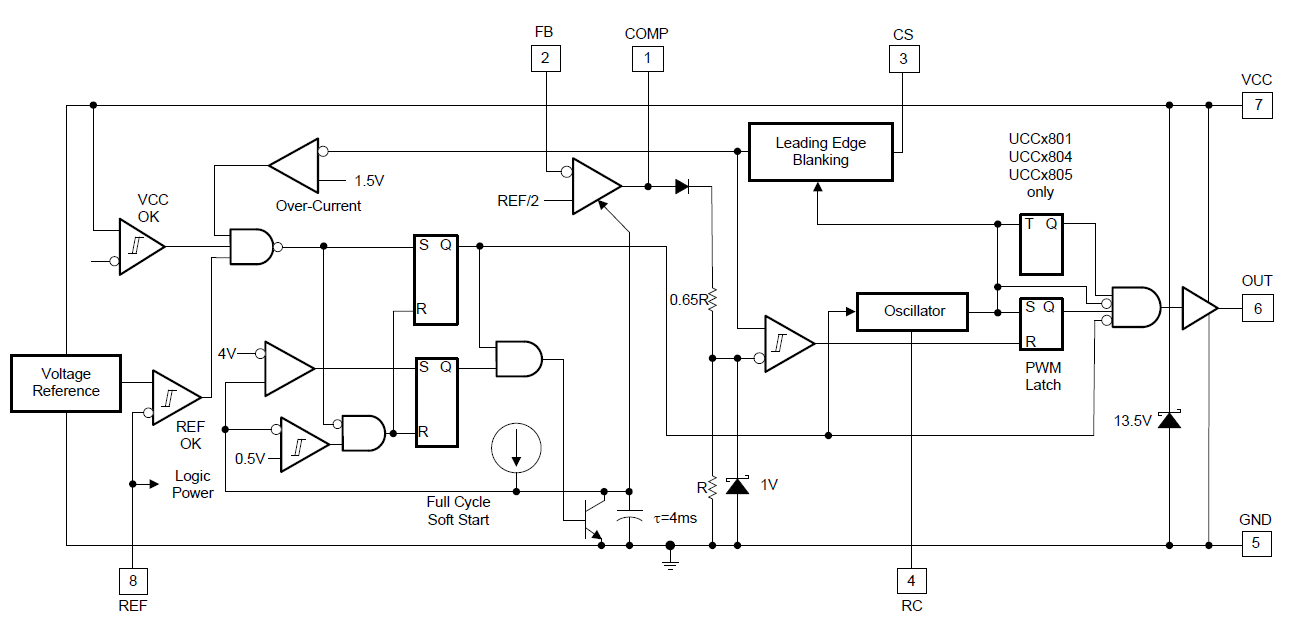
\includegraphics[width=1\linewidth]{../Dokumentation/tex/2iteration/billeder/PWM_block_diagram.png}
	\caption{Block diagram UCC1801}
	\label{fig:PWM_diagram}
\end{figure}

UCC1801 understøtter peak-current regulering, ved at indeholde to reguleringssløjfer i form af en fejlforstærker og en komparator. Fejlforstærkeren regulerer efter udgangsspændingen, mens komparatoren regulerer efter peak-strømmen i transformatorens primærvikling. Udgangen fra fejlforstærkeren sætter referenceværdien til komparatoren, som derfor bestemmer hvor langt strømmen vil rampe op, før komparatoren inverterer udgangssignalet. Når længden af switch-perioden er opnået vil et oscillator kredsløb i controlleren invertere udgangssignalet igen, hvorved det variable PWM-signal opnås. 

En anden fordel ved denne controller er, den indeholder en soft-start funktion, kaldet UVLO. Dette beskytter converteren, hvis forsyningen på PWM-controlleren er for lav til at drive MOSFET'en. Ved UCC1801 tvinger UVLO udgangen lav, hvis forsyningsspændingen er mindre end $9.4V$.

PWM-signalets switch-frekvens sættes ved tidskonstanten for et eksternt RC-netværk. Det generer en stigende spænding, da kondensatoren oplades. Denne spænding er forbundet til et komparator kredsløb internt i controlleren, som aflader kondensatoren gennem en transistor når komparatorens maksimale spænding er opnået. På grund af en hurtigere afladning- end opladningstid i kondensatoren vil dette genere en savtandspænding. Frekvensen af dette signal skal være den dobbelte af den ønskede switch-frekvens. Derfor kan modstanden beregnes til $R_T = 33.2k\ohm$, når kondensatoren er valgt til $200pF$.

Komparatoren der skal skifte på current-sense signalet, inverterer udgangen ved en peak-spænding på $1V$. Derfor skal der bruges en modstand, til at omsætte strømmen i primærviklingen til en spænding. Da komparatoren skifter ved en peak-spænding på $1V$, skal dette niveau svare til den ønskede peak-strøm i primærviklingen. Her bruges Ohm's lov til at beregne impedans på $R_{cs} = 0.181\ohm$. Denne modstand er blevet realiseret ved $6\cdot 1\ohm$ i paralle, og derfor også afrundet til $0.167\ohm$. 

På grund af switching-spikes i MOSFET'en, kan komparatoren skifte på disse spikes, hvis de svare til en spænding over modstanden større end $1V$. Derfor er der blevet designet et RC-filter, for begrænsning af current-sense signalets stigetid. I controlleren er der integreret et digitalt filter, som filtrer de første $100ns$. Derfor blev det eksterne filter designet til en stigetid på $300ns$. Her blev modstanden regnet til $R_f = 1.4k\ohm$, ved en kondensator på $100pF$.

Fejlforstærkeren er forbundet til en referencespænding på $2.5V$. Derfor blev der designet en spændingsdeler, for at dele udgangsspændingen ned. Her blev $R_{FB1}$ regnet til $18.7k\ohm$, og $R_{FB2}$ blev regnet til en parallelforbindelse mellem $2.55k\ohm$ og $280k\ohm$. 


For at kunne simulere PWM-controllerens funktionaliteter, blev der hentet en p-spice model for denne, ved Texas Instruments\cite{ucc1801-pspice}. Det samlede kredsløb for PWM-controlleren er vist på figur~\ref{fig:PWM_sim_diagram}.

\begin{figure}[H]
	\centering
	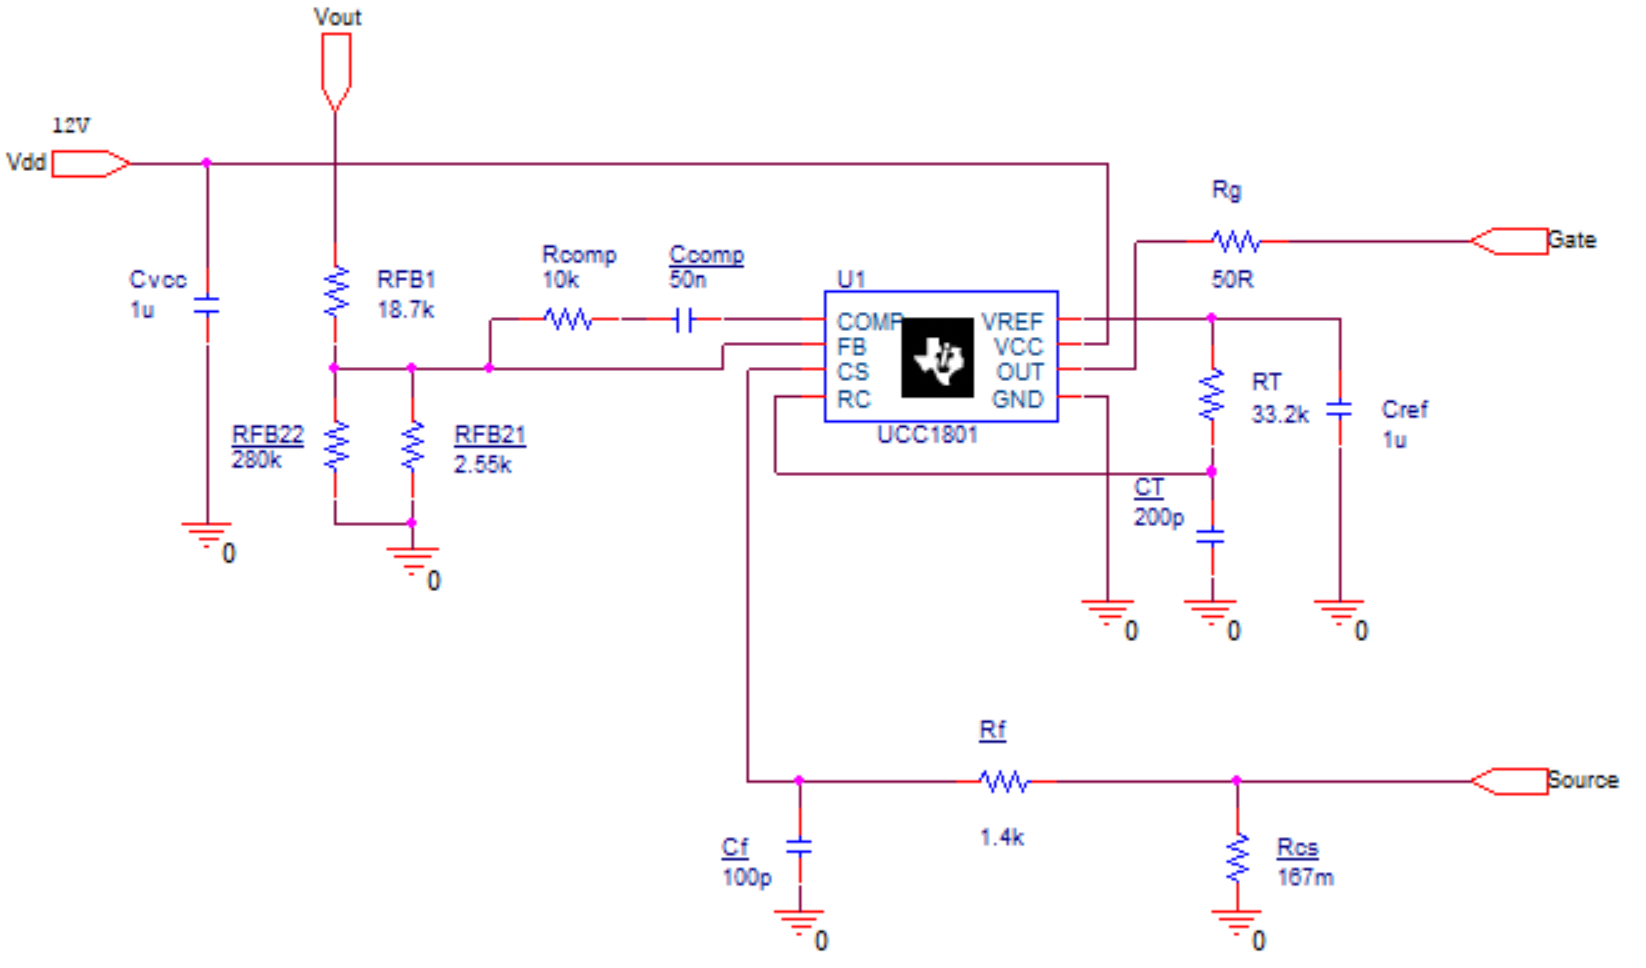
\includegraphics[width=0.9\linewidth]{/tex/Implementering/2iteration/billeder/PWM_diagram.png}
	\caption{Diagram for PWM-kredsløb}
	\label{fig:PWM_sim_diagram}
\end{figure} 

En mere detaljeret gennemgang af PWM-controllerens funktionaliteter og design af disse, er beskrevet i dokumentationens afsnit 5.2.

